\documentclass[8pt,apectratio=169]{beamer}

\usetheme[progressbar=frametitle]{metropolis}
\usepackage{appendixnumberbeamer}
\usepackage[style=authoryear, backend=bibtex8, natbib=true, maxcitenames=2]{biblatex}

\usepackage[utf8]{inputenc} % utf8x  defines more symbols, but may cause compatible problems
\usepackage{lmodern,textcomp} % Latin Modern fonts, contains €

\usepackage{graphicx}
\usepackage{import}

\usepackage{booktabs}
\usepackage[scale=2]{ccicons}

\usepackage{pgfplots}
\usepgfplotslibrary{dateplot}

\usepackage{xspace}
\newcommand{\themename}{\textbf{\textsc{metropolis}}\xspace}

% Math
\usepackage{amsmath}
\usepackage{bm} % bold symbol in math mode

% Optional packages
\usepackage{xcolor}
\usepackage{multicol}
\usepackage{hyperref}
\usepackage[super,negative]{nth} % allows writing 1st, 2nd, 3rd with superscript
\usepackage{ulem} % use the "sout" tag to "strikethrough" text
\usepackage{tcolorbox}

% Select what to do with command \comment:
  % \newcommand{\comment}[1]{}  %comments not shown
  % \newcommand{\comment}[1]{\par {\bfseries \color{blue} #1 \par}} %comments shown
% Select what to do with todonotes: i.e. \todo{}, \todo[inline]{}
  % \usepackage[disable]{todonotes} % notes not shown
  % \usepackage[draft]{todonotes}   % notes shown

%\numberwithin{equation}{section}

%\addbibresource{references}

\titlegraphic{\hfill 
\includegraphics[width=0.15 \textwidth]{figures/logo}}
\title{Microeconomics III, Ex. Class 4: Problem Set 1\footnote{Slides created for exercise class 4, with reservation for possible errors.\\}}
\author{Thor Donsby Noe (\href{mailto:thor.noe@econ.ku.dk}{thor.noe@econ.ku.dk})}
\date{September 11 2019} % \today
\institute{\normalsize Department of Economics, University of Copenhagen}

    % \definecolor{BlueTOL}{HTML}{222255}
    \definecolor{BrownTOL}{HTML}{666633}
    \definecolor{GreenTOL}{HTML}{225522}
    % \setbeamercolor{normal text}{fg=BlueTOL,bg=white}
    \setbeamercolor{alerted text}{fg=BrownTOL}
    \setbeamercolor{example text}{fg=GreenTOL}
    \setbeamercolor{background canvas}{bg=white}

    \setbeamercolor{block title alerted}{use=alerted text,
        fg=alerted text.fg,
        bg=alerted text.bg!80!alerted text.fg}
    \setbeamercolor{block body alerted}{use={block title alerted, alerted text},
        fg=alerted text.fg,
        bg=block title alerted.bg!50!alerted text.bg}
    \setbeamercolor{block title example}{use=example text,
        fg=example text.fg,
        bg=example text.bg!80!example text.fg}
    \setbeamercolor{block body example}{use={block title example, example text},
        fg=example text.fg,
        bg=block title example.bg!50!example text.bg}

\begin{document}
\maketitle

% ------------------------------------------------------------------------------
% ------ FRAME -----------------------------------------------------------------
% ------------------------------------------------------------------------------
\begin{frame}{Outline}
    \tableofcontents
\end{frame}

\section{PS4, Ex. 1 (A): MSNE and best-response functions}

\begin{frame}{Kahoot: PS4, Ex. 1 (A): MSNE and best-response functions}
  Form a group for each table:
  \begin{itemize}
    \item Get prepared to answer exercise 1 in problem set 4 as a team (5 min).
  \end{itemize}
  
\includegraphics[width=\textwidth]{figures/kahoot}
\end{frame}
\begin{frame}{PS4, Ex. 1 (A): MSNE and best-response functions}
  Find all equilibria (pure and mixed) in the following games, first analytically and then through plotting the best-response functions.
  \begin{multicols}{2}
    \begin{itemize}
      \item[(a)]
    \end{itemize}
    \begin{table}
      \begin{tabular}{cl|c|c|}
          & \multicolumn{1}{c}{} & \multicolumn{2}{c}{Player 2}\\
          \parbox[t]{1mm}{\multirow{3}{*}{\rotatebox[origin=r]{90}{Player 1}}}
          & \multicolumn{1}{c}{} & \multicolumn{1}{c}{L (q)} & \multicolumn{1}{c}{L (1-q)} \\\cline{3-4}
          & T (p) & 3, 3 & 0, 0 \\\cline{3-4}
          & B (1-p) & 0, 0 & 4, 4 \\\cline{3-4}
      \end{tabular}
    \end{table}
  \vfill\null \columnbreak
    \begin{itemize}
      \item[(b)]
    \end{itemize}
    \begin{table}
      \begin{tabular}{cl|c|c|}
          & \multicolumn{1}{c}{} & \multicolumn{2}{c}{Player 2}\\
          \parbox[t]{1mm}{\multirow{3}{*}{\rotatebox[origin=r]{90}{Player 1}}}
          & \multicolumn{1}{c}{} & \multicolumn{1}{c}{L (q)} & \multicolumn{1}{c}{L (1-q)} \\\cline{3-4}
          & T (p) & 1, 1 & 0, 0 \\\cline{3-4}
          & B (1-p) & 1, 0 & 2, 1 \\\cline{3-4}
      \end{tabular}
    \end{table}
  \vfill\null
  \end{multicols}
\end{frame}
\begin{frame}{PS4, Ex. 1 (A): MSNE and best-response functions}
  \begin{multicols}{2}
    \begin{itemize}
      \item[(a)] Find all equilibria (pure and mixed), first analytically and then through plotting the BR functions.
    \end{itemize}
    \begin{table}
      \begin{tabular}{cl|c|c|}
        & \multicolumn{1}{c}{} & \multicolumn{2}{c}{\color{blue}Player 2}\\
        \parbox[t]{1mm}{\multirow{3}{*}{\rotatebox[origin=r]{90}{\color{red}Player 1}}}
        & \multicolumn{1}{c}{} & \multicolumn{1}{c}{L (q)} & \multicolumn{1}{c}{L (1-q)} \\\cline{3-4}
        & T (p) & \textcolor{red}{3}, \textcolor{blue}{3} & 0, 0 \\\cline{3-4}
        & B (1-p) & 0, 0 & \textcolor{red}{4}, \textcolor{blue}{4} \\\cline{3-4}
      \end{tabular}
    \end{table}
    Find $q$ such that Player 1 expect to have equal payoffs from playing $T$ and $B$:
    \begin{align*}
      E[u_1|T]&=E[u_1|B]\\
      3q &= 4(1-q) \Rightarrow q = \frac{4}{7}
    \end{align*}
    The players have symmetric payoffs, thus:
    \begin{align*}
      NE=(p^{*},q^{*})=\left\{(0,0);\left(\frac{4}{7},\frac{4}{7}\right);(1,1)\right\}
    \end{align*}
  \vfill\null \columnbreak
    Plot the BR functions:
    \vspace{-8pt}
    \begin{align*}
      BR_1(q)=\left\{ \begin{array}{lcl}
          p=0       & \text{if} & q<4/7 \\
          p\in[0,1] & \text{if} & q=4/7 \\
          p = 1     & \text{if} & q>4/7
      \end{array}\right. \\
      BR_2(p)=\left\{ \begin{array}{lcl}
          q=0       & \text{if} & p<4/7  \\
          q\in[0,1] & \text{if} & p=4/7 \\
          q = 1     & \text{if} & p>4/7
      \end{array}\right.
    \end{align*}
    \vspace{-8pt}
    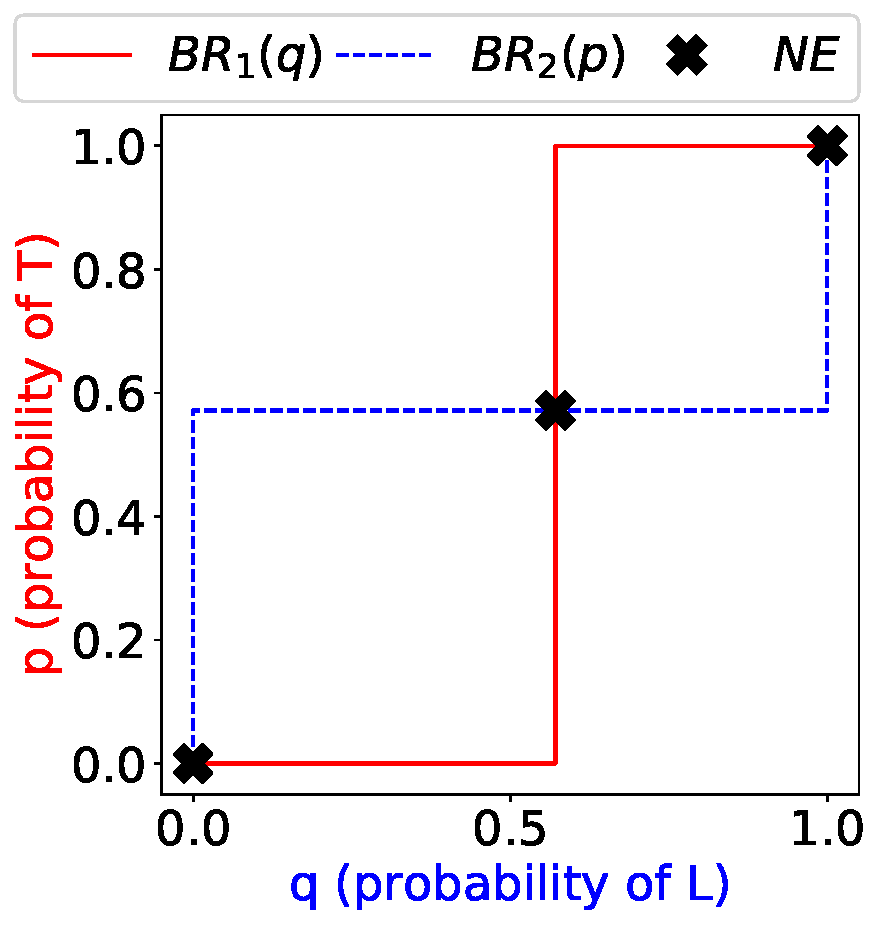
\includegraphics[width=\columnwidth]{figures/1a}
  \vfill\null
  \end{multicols}
\end{frame}
\begin{frame}{PS4, Ex. 1 (A): MSNE and best-response functions}
  \begin{multicols}{2}
    \begin{itemize}
      \item[(b)] Find all NE, first analytically:
    \end{itemize}
    \begin{table}
      \begin{tabular}{cl|c|c|}
        & \multicolumn{1}{c}{} & \multicolumn{2}{c}{\color{blue}Player 2}\\
        \parbox[t]{1mm}{\multirow{3}{*}{\rotatebox[origin=r]{90}{\color{red}Player 1}}}
        & \multicolumn{1}{c}{} & \multicolumn{1}{c}{L (q)} & \multicolumn{1}{c}{L (1-q)} \\\cline{3-4}
        & T (p) & \textcolor{red}{1}, \textcolor{blue}{1} & 0, 0 \\\cline{3-4}
        & B (1-p) & \textcolor{red}{1}, 0 & \textcolor{red}{2}, \textcolor{blue}{1} \\\cline{3-4}
      \end{tabular}
    \end{table}
    Player 1 is indifferent for:
    \begin{align*}
      E[u_1|T]&=E[u_1|B]\\
      q &= q + 2(1-q) \Rightarrow q = 1
    \end{align*}
    Player 2 is indifferent for:
    \begin{align*}
      E[u_2|L]&=E[u_2|R]\\
      p &= 1-p \Rightarrow p = \frac{1}{2}
    \end{align*}
    The pure and mixed strategy NE are:
    \begin{align*}
      NE:\left\{(0,0);(1,1);\left(p\in\left[\frac{1}{2},1\right),q=1\right)\right\}
    \end{align*}
  \vfill\null \columnbreak
    Then through plotting the BR functions:
    \vspace{-8pt}
    \begin{align*}
      BR_1(q)=\left\{ \begin{array}{lcl}
          p=0       & \text{if} & q<1 \\
          p\in[0,1] & \text{if} & q=1
      \end{array}\right. \\
      BR_2(p)=\left\{ \begin{array}{lcl}
          q=0       & \text{if} & p<1/2  \\
          q\in[0,1] & \text{if} & p=1/2 \\
          q=1       & \text{if} & p>1/2
      \end{array}\right.
    \end{align*}
    \vspace{-8pt}
    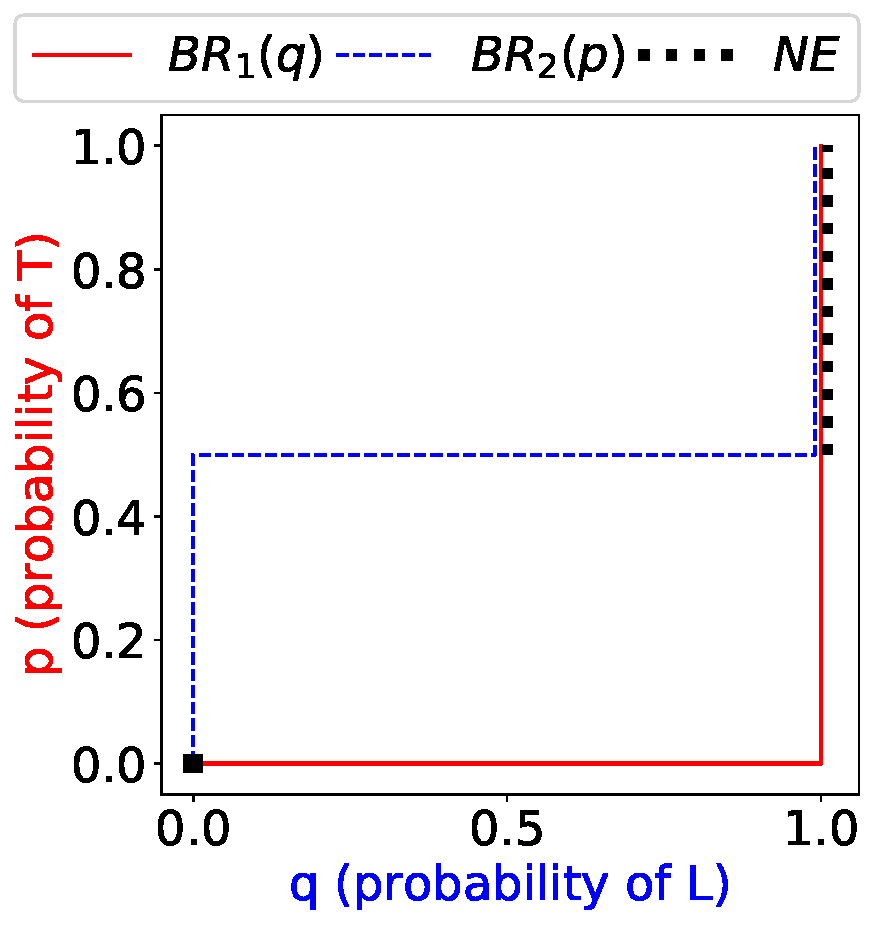
\includegraphics[width=\columnwidth]{figures/1b}
  \vfill\null
  \end{multicols}
\end{frame}








\section{PS4, Ex. 3: }

\begin{frame}{PS4, Ex. 3: }

\end{frame}


\section{PS4, Ex. 4: }

\begin{frame}{PS4, Ex. 4: }

\end{frame}


\section{PS4, Ex. 5: }

\begin{frame}{PS4, Ex. 5: }

\end{frame}


\section{PS4, Ex. 6: }

\begin{frame}{PS4, Ex. 6: }

\end{frame}


\section{PS4, Ex. 7: }

\begin{frame}{PS4, Ex. 7: }

\end{frame}


\section{Example slide with figures}

\begin{frame}{Example slide with figures}
  \begin{multicols}{2}
    \begin{table}
      \begin{tabular}{cl|c|c|}
          & \multicolumn{1}{c}{} & \multicolumn{2}{c}{Player 2}\\
          \parbox[t]{1mm}{\multirow{3}{*}{\rotatebox[origin=r]{90}{Player 1}}}
          & \multicolumn{1}{c}{} & \multicolumn{1}{c}{L (q)} & \multicolumn{1}{c}{L (1-q)} \\\cline{3-4}
          & T (p)   &  &  \\\cline{3-4}
          & B (1-p) &  &  \\\cline{3-4}
      \end{tabular}
    \end{table}
  \vfill\null \columnbreak
    \begin{table}
      \begin{tabular}{cc|c|c|}
        & \multicolumn{1}{c}{} & \multicolumn{2}{c}{\color{blue}Player 2}\\
        \parbox[t]{1mm}{\multirow{3}{*}{\rotatebox[origin=r]{90}{\color{red}Player 1}}}
        & \multicolumn{1}{c}{} & \multicolumn{1}{c}{L (q)} & \multicolumn{1}{c}{L (1-q)} \\\cline{3-4}
        & T (p)   & \textcolor{red}{}, \textcolor{blue}{} &   \\\cline{3-4}
        & B (1-p) &  &  \\\cline{3-4}
      \end{tabular}
    \end{table}
    \begin{table}
      \begin{tabular}{l|c|c|}
          \multicolumn{1}{c}{} & \multicolumn{1}{c}{L (q)} & \multicolumn{1}{c}{L (1-q)} \\\cline{2-3}
          T (p)   &  &  \\\cline{2-3}
          B (1-p) &  &  \\\cline{2-3}
      \end{tabular}
    \end{table}
  \vfill\null
  \end{multicols}
\end{frame}


\section{PS3, Ex. 5: Luxembourg as a rogue state}

\begin{frame}{PS3, Ex. 5: Luxembourg as a rogue state}
  \begin{multicols}{2}
    Assume that Luxembourg has turned into a rogue state. It is close to acquiring nuclear weapons, which would threaten the stability in the whole region. The Vatican ($V$) and Denmark ($D$) are preparing an attack on Luxembourg’s nuclear research facilities to stop or slow down its nuclear program. The probability that the attack will be a success is
    \begin{align*}
      p(s_V,s_D)=s_V+s_D-s_vs_D,
    \end{align*}
    where $s_i\in[0,1]$ is the share of its military capacity that country $i\ (i\in\{V,D\})$ uses in the attack. If the attack is successful then each country receives a payoff of 1. The cost of participating in the attack for country $i$ is
    \begin{align*}
      c_i(s_i)=s_i^2
    \end{align*}
    The objective of each country is to maximize its expected payoff from the attack minus the cost.
  \vfill\null\columnbreak
    \begin{itemize}
      \item[(a)] Suppose that the Vatican and Denmark choose the shares of military capacity to use in the attack simultaneously and independently. Find the Nash equilibrium (NE) of this game.
      \item[(b)] Find the social optimum (SO) under the condition that the two countries use the same share of their military capacity. I.e., find the $\bar{s}_V=\bar{s}_D=\bar{s}$ that maximizes aggregate payoff from the attack minus costs. Compare with the equilibrium from question (a) and give an intuitive explanation of your findings.
    \end{itemize}
    \hfill 
\includegraphics[width=0.20 \textwidth]{figures/nuclear}
  \vfill\null
  \end{multicols}
\end{frame}
\begin{frame}{PS3, Ex. 5: Luxembourg as a rogue state}
  \begin{multicols}{2}
    \begin{itemize}
      \item[(a)] Find the NE in the static game:
    \end{itemize}
    Expected payoff for player $i\neq j$:
    \begin{align*}
      u_i(s_i,s_j)=\underbrace{s_i+s_j-s_is_j}_\text{Probability of success}-\underbrace{s_i^2}_\text{Cost}
    \end{align*}
  \vfill\null\columnbreak
  \vfill\null
  \end{multicols}
\end{frame}
\begin{frame}{PS3, Ex. 5: Luxembourg as a rogue state}
  \begin{multicols}{2}
    \begin{itemize}
      \item[(a)] Find the NE in the static game:
    \end{itemize}
    Expected payoff for player $i\neq j$:
    \begin{align*}
      u_i(s_i,s_j)=\underbrace{s_i+s_j-s_is_j}_\text{Probability of success}-\underbrace{s_i^2}_\text{Cost}
    \end{align*}
    Find the best-response function for $i$:
    \begin{align*}
      FOC:\ \frac{\delta u_i}{\delta s_i}=1+0-s_j-2s_i&=0\\
       s_i&=\frac{1-s_j}{2}
    \end{align*}
  \vfill\null\columnbreak
  \vfill\null
  \end{multicols}
\end{frame}
\begin{frame}{PS3, Ex. 5: Luxembourg as a rogue state}
  \begin{multicols}{2}
    \begin{itemize}
      \item[(a)] Find the NE in the static game:
    \end{itemize}
    Expected payoff for player $i\neq j$:
    \begin{align*}
      u_i(s_i,s_j)=\underbrace{s_i+s_j-s_is_j}_\text{Probability of success}-\underbrace{s_i^2}_\text{Cost}
    \end{align*}
    Find the best-response function for $i$:
    \begin{align*}
      FOC:\ \frac{\delta u_i}{\delta s_i}=1+0-s_j-2s_i&=0\\
       s_i&=\frac{1-s_j}{2}
    \end{align*}
    Taking advantage of symmetry $s_i^{*}=s_j^{*}$:
    \begin{align*}
       s_i^{*}&=\frac{1-s_i^{*}}{2}\\
      2s_i^{*}+s_i^{*}&=1\\
       s_i^{*}&=\frac{1}{3}\equiv s^{NE}
    \end{align*}
    i.e. $NE=\left\{(s_D^{*},s_V^{*})=(\frac{1}{3},\frac{1}{3})\right\}$
  \vfill\null\columnbreak
  \vfill\null
  \end{multicols}
\end{frame}
\begin{frame}{PS3, Ex. 5: Luxembourg as a rogue state}
  \begin{multicols}{2}
    \begin{itemize}
      \item[(a)] Find the NE in the static game:
    \end{itemize}
    Expected payoff for player $i\neq j$:
    \begin{align*}
      u_i(s_i,s_j)=\underbrace{s_i+s_j-s_is_j}_\text{Probability of success}-\underbrace{s_i^2}_\text{Cost}
    \end{align*}
    Find the best-response function for $i$:
    \begin{align*}
      FOC:\ \frac{\delta u_i}{\delta s_i}=1+0-s_j-2s_i&=0\\
       s_i&=\frac{1-s_j}{2}
    \end{align*}
    Taking advantage of symmetry $s_i^{*}=s_j^{*}$:
    \begin{align*}
       s_i^{*}&=\frac{1-s_i^{*}}{2}\\
      2s_i^{*}+s_i^{*}&=1\\
       s_i^{*}&=\frac{1}{3}\equiv s^{NE}
    \end{align*}
    i.e. $NE=\left\{(s_D^{*},s_V^{*})=(\frac{1}{3},\frac{1}{3})\right\}$
  \vfill\null\columnbreak
    \begin{itemize}
      \item[(b)] Find the SO given shares are equal:
    \end{itemize}
  \vfill\null
  \end{multicols}
\end{frame}
\begin{frame}{PS3, Ex. 5: Luxembourg as a rogue state}
  \begin{multicols}{2}
    \begin{itemize}
      \item[(a)] Find the NE in the static game:
    \end{itemize}
    Expected payoff for player $i\neq j$:
    \begin{align*}
      u_i(s_i,s_j)=\underbrace{s_i+s_j-s_is_j}_\text{Probability of success}-\underbrace{s_i^2}_\text{Cost}
    \end{align*}
    Find the best-response function for $i$:
    \begin{align*}
      FOC:\ \frac{\delta u_i}{\delta s_i}=1+0-s_j-2s_i&=0\\
       s_i&=\frac{1-s_j}{2}
    \end{align*}
    Taking advantage of symmetry $s_i^{*}=s_j^{*}$:
    \begin{align*}
       s_i^{*}&=\frac{1-s_i^{*}}{2}\\
      2s_i^{*}+s_i^{*}&=1\\
       s_i^{*}&=\frac{1}{3}\equiv s^{NE}
    \end{align*}
    i.e. $NE=\left\{(s_D^{*},s_V^{*})=(\frac{1}{3},\frac{1}{3})\right\}$
  \vfill\null\columnbreak
    \begin{itemize}
      \item[(b)] Find the SO given shares are equal:
    \end{itemize}
    Expected payoff for $i$, $\bar{s}_D=\bar{s}_V=\bar{s}$:
    \begin{align*}
      u_i(\bar{s})&=\underbrace{\bar{s}+\bar{s}-\bar{s}\bar{s}}_\text{Probability of success}-\underbrace{\bar{s}^2}_\text{Cost}\\
                  &=2\bar{s}-2\bar{s}^2
    \end{align*}
  \vfill\null
  \end{multicols}
\end{frame}
\begin{frame}{PS3, Ex. 5: Luxembourg as a rogue state}
  \begin{multicols}{2}
    \begin{itemize}
      \item[(a)] Find the NE in the static game:
    \end{itemize}
    Expected payoff for player $i\neq j$:
    \begin{align*}
      u_i(s_i,s_j)=\underbrace{s_i+s_j-s_is_j}_\text{Probability of success}-\underbrace{s_i^2}_\text{Cost}
    \end{align*}
    Find the best-response function for $i$:
    \begin{align*}
      FOC:\ \frac{\delta u_i}{\delta s_i}=1+0-s_j-2s_i&=0\\
       s_i&=\frac{1-s_j}{2}
    \end{align*}
    Taking advantage of symmetry $s_i^{*}=s_j^{*}$:
    \begin{align*}
       s_i^{*}&=\frac{1-s_i^{*}}{2}\\
      2s_i^{*}+s_i^{*}&=1\\
       s_i^{*}&=\frac{1}{3}\equiv s^{NE}
    \end{align*}
    i.e. $NE=\left\{(s_D^{*},s_V^{*})=(\frac{1}{3},\frac{1}{3})\right\}$
  \vfill\null\columnbreak
    \begin{itemize}
      \item[(b)] Find the SO given shares are equal:
    \end{itemize}
    Expected payoff for $i$, $\bar{s}_D=\bar{s}_V=\bar{s}$:
    \begin{align*}
      u_i(\bar{s})&=\underbrace{\bar{s}+\bar{s}-\bar{s}\bar{s}}_\text{Probability of success}-\underbrace{\bar{s}^2}_\text{Cost}\\
                  &=2\bar{s}-2\bar{s}^2
    \end{align*}
    Social planner target function:
    \begin{align*}
      \pi^S(\bar{s})&=\underbrace{2}_\text{Countries}(2\bar{s}-2\bar{s}^2)=4\bar{s}-4\bar{s}^2
    \end{align*}
  \vfill\null
  \end{multicols}
\end{frame}
\begin{frame}{PS3, Ex. 5: Luxembourg as a rogue state}
  \begin{multicols}{2}
    \begin{itemize}
      \item[(a)] Find the NE in the static game:
    \end{itemize}
    Expected payoff for player $i\neq j$:
    \begin{align*}
      u_i(s_i,s_j)=\underbrace{s_i+s_j-s_is_j}_\text{Probability of success}-\underbrace{s_i^2}_\text{Cost}
    \end{align*}
    Find the best-response function for $i$:
    \begin{align*}
      FOC:\ \frac{\delta u_i}{\delta s_i}=1+0-s_j-2s_i&=0\\
       s_i&=\frac{1-s_j}{2}
    \end{align*}
    Taking advantage of symmetry $s_i^{*}=s_j^{*}$:
    \begin{align*}
       s_i^{*}&=\frac{1-s_i^{*}}{2}\\
      2s_i^{*}+s_i^{*}&=1\\
       s_i^{*}&=\frac{1}{3}\equiv s^{NE}
    \end{align*}
    i.e. $NE=\left\{(s_D^{*},s_V^{*})=(\frac{1}{3},\frac{1}{3})\right\}$
  \vfill\null\columnbreak
    \begin{itemize}
      \item[(b)] Find the SO given shares are equal:
    \end{itemize}
    Expected payoff for $i$, $\bar{s}_D=\bar{s}_V=\bar{s}$:
    \begin{align*}
      u_i(\bar{s})&=\underbrace{\bar{s}+\bar{s}-\bar{s}\bar{s}}_\text{Probability of success}-\underbrace{\bar{s}^2}_\text{Cost}\\
                  &=2\bar{s}-2\bar{s}^2
    \end{align*}
    Social planner target function:
    \begin{align*}
      \pi^S(\bar{s})&=\underbrace{2}_\text{Countries}(2\bar{s}-2\bar{s}^2)=4\bar{s}-4\bar{s}^2
    \end{align*}
    Find the social optimum (SO):
    \begin{align*}
      FOC:\ \frac{\delta\pi^S}{\delta s_i}=4-8\bar{S}&=0\\
       \bar{S}&=\frac{4}{8}=\frac{1}{2}>\frac{1}{3}
    \end{align*}
    i.e. the SO is higher than the NE as the positive externality is not rewarded, leading to an incentive to free ride.
  \vfill\null
  \end{multicols}
\end{frame}


\section{PS4, Ex. 8: Stackelberg}

\begin{frame}{PS4, Ex. 8: Stackelberg}

\end{frame}



\end{document}
